\documentclass[12pt]{article}
\usepackage[margin=1in]{geometry}
\usepackage{hyperref}
\usepackage{verbatim}
\usepackage{graphicx}

%%%%%%%%%%%%%%%%%%%%%%%%%%%%%%%%%%%%%%%%%%%%%%%%%%%%%%%%%%%%%%%%%%%%%%%
\def\sentence#1{\par\noindent\textbf{#1}}
%%%%%%%%%%%%%%%%%%%%%%%%%%%%%%%%%%%%%%%%%%%%%%%%%%%%%%%%%%%%%%%%%%%%%%%

\title{COPTIC Reference Manual}
\author{I H Hutchinson}
\begin{document}
\maketitle
\begin{abstract}
  
  This manual documents the particle-in-cell code COPTIC. COPTIC is a
  cartesian-mesh, oblique-boundary, particles and thermals in cell
  code.  It moves particles in three dimensions of space and time (6
  phase-space dimensions) and simultaneously calculates the
  self-consistent electrostatic potential in the presence of a
  neutralizing species governed by a thermal Boltzmann factor, or of a
  second particle species. Normally the first species is ions and the
  second electrons; but various other options are possible.  An
  arbitrary uniform magnetic field can be applied.  Objects of various
  shapes on which boundary conditions can be specified can be placed
  in the computational domain, and can be used to define the plasma
  domain. Various options also exist for simulating open or periodic
  domains with various velocity distributions. A particular facility
  is to initialize the plasma with a self consistent electron hole,
  whose evolution can then be simulated.  The code is substantially
  self-documenting through comments, but the manual ought to assist a
  newcomer with fuller explanations. To run the code, the material of
  sections \ref{infile} and \ref{cmdline} are sufficient. Subsequent
  sections describe the structure of the code and how it works.
\end{abstract}


\tableofcontents


\section{Object Data and Geometry Input File}\label{infile}

COPTIC acquires its settings from a combination of command line
arguments and an input file that gives information about geometry,
which is referred to as the object file.  The purpose of this section
is to explain the format and meaning of the object file. Some
parameters are set either in the object file or by command line
arguments. A command line argument always overrides the object file.


\paragraph{The default name} of the input file is \verb!copticgeom.dat!, but it
may be set to any other name by a non-switch commandline argument
(something not starting \verb!-!), or using the command line object file
switch in the form \verb!-ofNewFileName.Ext!.

\subsection{Overall format}

\paragraph{Each line of the object file} is treated separately: read and parsed to
extract its settings. If COPTIC does not reach the end of the file
because it encounters an error in reading or parsing before that, then
it stops with an error message.

\paragraph{Comment lines.} A line that starts with a hash (\#) 
or with 6 or more spaces, or is blank is ignored as a
comment. Comments can also be placed at the right-hand end of data
lines that provide all the data that is expected of a line of that
type. Some types of line can be written short: without providing some
optional data. A comment cannot be placed at the end of a short line.
It is better for most object lines to avoid trailing comments.

\paragraph{The first line} Is always a comment. Nothing on this line is used.

\paragraph{Argument lines.} Any line that begins \verb!Arguments:! is
regarded as an argument line, and is stored, adding to any earlier
such argument lines. The text following the colon is parsed for
additional command line switches before starting on the actual command
line arguments. This makes it possible, if desired, to put all of the
settings that control a run into a single object file, and require no
switches explicitly on the command line. Obviously the exception to
this ability is that the name of the object file cannot be set in the
object file!

\subsection{Object Lines}

Objects in coptic are represented by a ``constructive geometry''
approach. That is, they are composed of a small number of simple
shapes that can be added or subtracted rather than by general objects
with arbitrary numbers of faces, vertices, etc. The major advantage of
the constructive approach is that it is easy and quick to determine
whether any arbitrary position is inside or outside the object(s).

\paragraph{The format} of an object line is a sequence of numbers
separated by standard fortran separators (blanks, commas, or
semicolons). For actual objects, these are read as reals into a data
structure \verb!obj_geom(i,nobj)! whose first index refers to the
different values, and whose second refers to the object number
($\le31$ at present).  Some of the numbers are expected to be integers
but it does not matter if they are written as reals. The position in
the first index of \verb!obj_geom(i,nobj)!, i.e.\ the value of
\verb!i!, is referred to using a number of pre-defined integer
parameters (defined in \verb!3dcom.f!), most of which begin with the
letter \verb!o!. There is overloading of the positions, with different
parameters for different types of line. The index parameters are
mentioned below.

\paragraph{The first entry} 
\verb!obj_geom(otype,iobj)! of every object line is an integer which
determines the type of line this is, what sort of object or other
entity it refers to. The first byte specifies the object type and the
second byte further qualifies it. The parameters are specified with
\emph{required} subsequent values as follows:

\paragraph{1 Spheroid}: position of center and three radii in the
direction of the coordinate axes.

\paragraph{2 Cuboid (coordinate aligned)}: center and three
half-side-lengths, so that the cube extends in each coordinate
direction from center minus half-side-length to center plus
half-side-length.

\paragraph{3 Cylinder (coordinate aligned)}: center, three ``radii''
along the respective coordinates, axis-number specifying the
coordinate along which the cylinder's axis is aligned. For this
direction the ``radius'' is the cylinder's half-length.

\paragraph{4 Parallelopiped}: center ${\bf x}_c$, and three vectors
${\bf v}_k$ specifying the
direction and half-length of the parallelopiped's edges. The volume
consists of those points whose vectorial position can be expressed as
\begin{equation}\label{parallelocoef}
{\bf x} = {\bf x}_c + \sum_k^3 c_k {\bf v}_k,  
\end{equation}
with each coefficient
$c_k$ satisfying $-1\le c_k \le 1$. A non-aligned cuboid (for example)
is a
particular case of the parallelopiped. 

\paragraph{5 Cylinder (non-aligned)}: center, axis-vector specifying the
direction and half-length of the cylinder's axis, reference-vector
whose direction perpendicular to the axis-vector specifies the
direction from which angles in the cylinder are to be measured, and
radius. (This specifies only circular cross-section cylinders. It is a
special case of a surface of revolution below, but with slightly
easier entry and slightly faster performance.)

\paragraph{6 Surface-of-Revolution (monotonic convex)}: base, apex
position-vectors specifying the axis of revolution and the start and
end points of the surface; reference-vector whose component
perpendicular to axis gives the first coordinate direction in a
right-handed cartesian system of which the axis is the third
direction; radius-size being the length of unit radius in the radial
point specification; \verb!npair! the number of subsequent (r,z)
pairs; then \verb!npair! pairs of cylindrical coordinates relative to
the specified axis consisting of axial z-positions (expressed as a
fractional distance between base and apex) and corresponding radial
r-values (normalized by radius-size) at each z. The z (fractional)
values must be monotonic between 0 and 1.

\paragraph{7 Surface-of-Revolution (general)}: base, apex specifying
axis of revolution; reference-vector; radius-size; \verb!npair! the
number of subsequent (r,z) pairs; then \verb!npair! pairs of
fractional z-positions (between base and apex) and corresponding
r-values at each z. The difference (from 6) is that all the points of the
surface must be specified as pairs; the z positions don't have to be
monotonic and may extend beyond the axis ends; and the surface must be
closed unless both ends are on the axis-line (r=0). [The maximum number
of pairs permitted for a surface of revolution is specified by
\verb!ovlen!, normally 20.]

\bigskip
For each object, the boundary conditions to be applied in the form 
$$A\phi + B \hat{\bf n}.\nabla\phi + C =0$$
are specified immediately after the type. If all of $A,B,C$ are zero,
then no potential boundary condition is applied on this object.

Examples of lines of each of these types are given in the following
extract suitably formatted to represent possible input lines.

\begin{verbatim}
# Spheroid
#type=1  A, B, C ,    Center,      Radii
1,       1.,0.,2.,  -2.,-2.,-2.,  1.,.5,1., 
# Cuboid
#type=2  A, B, C,     Center     Half-sides
2,       1.,0.,1.5,  2,-1,2,      1.,1.,1.
# Cylinder (Coordinate-aligned)
#type=3  A, B, C,     Center        Radii,  axial-direction. 
3,       1.,0.,1.,   0.,0.,0.,    1.,1.,1.,     3,
# Parallelopiped
#type=4  A, B, C,     Center      Vector1   Vector2    Vector3
4,       1.,0.,.5,  -2.,2.,-2.,   1.,0,.1,  -1.,0.,1., 0.,.7,0.
# Cylinder (Non-aligned)
#type=5  A, B, C,     Center      Axial-vec  Ref-vec   Radius
5,       1.,0.,1.,  2.,-2.,-2.,   1.,0.,1.,  1.,0.,0.,  1. ,
# Surface of Revolution (monotonic convex)
#type=6 A,B,C,   Base     Apex   Ref-Vec Rad Npair rz-Pairs (Npair in total)
6       1 0 1, 0. 0. -2, 0. 0. 2, 1 0 0, 1.,  4, 1. .01, .5 .4, .5 .7, .2 .9
# Surface of Revolution (general) (chosen to give same result)
#type=7 A,B,C,  Base  Apex Ref-Vec R Npair rz-Pairs (Npair in total)
7      1 0 1, 0 0 -2, 0 0 2, 1 0 0, 1,6,0 0, 1 .01, .5 .4, .5 .7, .2 .9, 0 1

\end{verbatim}

\subsection{Flux accumulation}

Optionally, every object line can include specification of the
accumulation of ion flux to its surface. This specification consists
of one integer specifying the number of types of flux (up to 5 at
present) to be accumulated, and then two or three integers defining
the way the surface is to be subdivided into bins in which the
accumulation takes place. The flux types are 1 ion-flux, 2-4
ion-momentum-flux in the coordinate directions, and 5 ion-energy-flux.

Subdivision of the object surface is into equal intervals of
appropriate surface-coordinates. Spheroid surfaces are subdivided
using just two directions, into equal-interval bins in cosine of the
polar angle ($\cos\theta$) relative to the $z$-coordinate, and
azimuthal angle $\psi$. These bins are therefore all the same
area for a sphere. Cylinder-surfaces are divided into equal-intervals of
cylindrical coordinates ($r,\theta,z$) relative to the cylinder's
axial direction, $z$. The cylinder faces (constant-$z$) are divided by
$r$ and $\theta$, while the curved cylinder surface is divided by
$\theta$ and $z$. Cuboidal or parallelopiped surfaces are divided
into equal intervals in the vector coefficients along the edges. In
other words, with reference to eq (\ref{parallelocoef}), the surfaces
at $c_1=\pm1$ are divided into equal intervals of $c_2$ and $c_3$, and
so forth. Spheroids therefore require two face-counts, which
correspond to the number of equal divisions of $\cos\theta$ and
$\psi$, while cylinders and parallelopipeds require three face-counts
specifying the number of facets in $r,\theta,z$ or $c_1,c_2,c_3$
respectively. For example.

\begin{verbatim}
# Spheroid that sets no potential BC but tracks flux across it.
#type=1  A, B, C ,    Center,      Radii  4 fluxes,8x8 angles
1,       0.,0.,0.,   0.,0.,7.5,  .5,.5,.5,     4,8,8
# Axis-aligned cylinder.
#type  A, B, C ,    Center,    Radii  Axis-3  1 flux r,th,z
3,     1.,0.,1.,   0.,0.,0.,  1.,1.,1., 3,    1,     2,3,5
# Parallelopiped
#  A, B, C,   Center       Vector2   Vector2   Vector3   Fluxes divisions
4, 1.,0.,.5,  -2.,2.,-2.,  1.,0,.1,  -1.,0.,1., 0.,.7,0.,    1,  2,2,2
# Non-aligned cylinder.
#  A, B, C,   Center      Axis      Ref-vec  radius  Fluxes  r,th,z
5, 1.,0.,1., 2.,-2.,-2., 1.,0.,1.,  1.,0.,0.,  1. ,    4,     2,3,4
\end{verbatim}

The numbers specifying the fluxes and surface facet divisions are
appended immediately after the geometry specification, on the same
line of the object file. For simple objects, there are three or four
numbers and they are stored in adjacent locations
\verb!obj_geom(i,iobj)! with \verb!i!  equal to \verb!ofluxtype!,
\verb!ofn1!, \verb!ofn2![, \verb!ofn3!].  [To leave room for other
information, \verb!ofluxtype!  is defined equal to \verb!oradius+20!.]
For surfaces of revolution, in addition to the fluxes and the
theta-divisions there are integers for each of the segments of the
contour of revolution, indicating into how many facets each is
divided. These specifications follow the (r,z) pairs that specify the
contour. All must be on the \emph{same unbroken} line in the
input file. For example a general contour with 5 pairs has 4 segments:
\begin{verbatim}
# General Surface of Revolution
#   ABC    Center... Npair... Fluxes th, n1,n2,n3,n4
7, 1 0 2, 0 0 0, ...  5   ...   1,   5,  4  4  10 1 
\end{verbatim}
Note that a type 6 surface of revolution has one \emph{more} segment
than specified point pairs (because the base and apex ends of the
axial vector are added), while a type 7 surface of revolution has one
\emph{less} segment than specified point pairs. 

Total flux to the object is always separately accumulated regardless
of the optional specification.  Therefore, it is not necessary to
specify the flux accumulation information unless measurement of the
flux as a function of \emph{subdivided} position on the object is
required. The signed flux for both directions of particle-crossing
is accumulated (positive inward, negative outward). 

If flux entering or leaving any region of the domain is required to be
monitored, then an object which represents the boundary of that region
should be defined with null boundary conditions. 

\subsection{Special Object Qualifications}

The second byte of the object type indicates special qualities of the
object as follows. 

\paragraph{1($\times256$) Special Boundary} for the outside region of this
object set the potential to zero at the boundary rather than the
normal continuity condition when a Robin form is used.

\paragraph{2($\times256=512$) Point-Charge} This spherical object is a
point charge, which is treated by the PPPM technique. Its potential is
represented by an analytic part that is non-zero out to a radius
specified as usual. Outside that (isotropic) radius, the analytic part
is zero. The magnitude of the point charge is specified by an input
value in the position of \verb!ofn1! (12th position in the object
line; the 11th position requires a number (0) but is ignored.) The
value at position \verb!ofn1! equals the Coulomb potential that would
exist at the object's radius if the charge were unshielded.
For example,
\begin{verbatim}
513, 0.,0.,0., 0.,1.,10.,  .4,.4,.4,  0,-1.,0
\end{verbatim}
denotes a point charge at position \verb!(0.,1.,10.)!, whose
analytic part extends to radius \verb!0.4!, and whose charge is such
that a pure Coulomb potential due to it would give rise to a potential
at \verb!0.4! of value \verb!-1.!\ (in other words its charge is
$0.4\times(-1.)\times4\pi$ normalized units). 

\paragraph{3($\times256=768$) Nonuniform Boundary Conditions} The
coefficients $A,B,C$ of the Robin boundary condition in this object vary
linearly in space. Their values at the object center are specified as
usual. Their gradients are specified by three vectors which follow the
flux accumulation specification (which must be present). The gradient
vectors are in reverse order: $C, B, A$, allowing just the C-vector
gradient components
$(x,y,z)$ to be specified if the other gradients are zero, which is
most often the case.

\paragraph{4($\times256=1024$) Insulating Object} The boundary
condition is the specification of the potential ($A,C\ne 0$). But the
value of $C$ is determined dynamically within the code by requiring
the value of the ion flux density to the local facet to equal the
electron flux density there.

\paragraph{5($\times256=1280$) Floating Object} The potential is constant
on the object, but takes a value determined by requiring the total ion
flux to the object to equal the electron flux.

\subsection{Object Subtraction}

More complicated concave-surface and hollow objects can be constructed
by subtraction of one object from another. When all (relevant) objects
have been defined by their object lines, a special object line with
\verb!otype! equal to 89 or 88 indicates subtraction. The type is
followed by an integer indicating the object (number) from which to
subtract (the ``additive'' object), an integer indicating how many
other objects are subtracted from it, N, and then N integers
indicating the ``subtractive'' objects' numbers O1, O2, ... ON. Thus lines
\begin{verbatim}
88, 1, 1, 2
89, 4, 2, 5, -6
\end{verbatim}
indicate respectively that object 1 has one object, namely object 2,
subtracted from it; while object 4 has two objects, 5 and -6
subtracted from it. A negative subtractive object means subtract the
\emph{complement}, i.e.\ the region outside the object, rather than
the inside.
\begin{figure}[htp]
\begin{minipage}{0.5\linewidth}{\tiny
\begin{verbatim}
//////////////////////////////// ////////////////////////////////
/~~~~~~~~~~~~~~~~~~~~~~~~~~~~~~/ /~~~~~~~~~~~~~~~~~~~~~~~~~~~~~~/
/~~~~~~~~~~~~~~~~~~~~~~~~~~~~~~/ /~~~~~~~~~~~~~~~~~~~~~~~~~~~~~~/
/~~~~~~~~~~~~~~~~~~~~~~~~~~~~~~/ /~~~~~~~~~~~~~~~~~~~~~~~~~~~~~~/
/~~~~~~~~~~~~~~~~~~~~~~~~~~~~~~/ /~~~~~~~~~~~~~~~~~~~~~~~~~~~~~~/
/~~~~~~~~~~~~~~~~~~~~~~~~~~~~~~/ /~~~~~~~~~~~~~~~~~~~~~~~~~~~~~~/
/~~~~~~~~~~~~~~~~~~~~~~~~~~~~~~/ /~~~~~~~~~~~~~~~~~~~~~~~~~~~~~~/
/~~~~~~~~~~~~~~~~~~~~~~~~~~~~~~/ /~~~~~~~~~~~~~~~~~~~~~~~~~~~~~~/
/~~~~~~~~~~~~~~~~~~~~~~~~~~~~~~/ /~~~~~~~~~~~~~~~~~~~~~~~~~~~~~~/
/~~~~~~~~~~~00000000~~~~~~~~~~~/ /~~~~~~~~~~~00000000~~~~~~~~~~~/
/~~~~~~~~~000111111000~~~~~~~~~/ /~~~~~~~~~000111111000~~~~~~~~~/
/~~~~~~~~~0111~~~~1110~~~~~~~~~/ /~~~~~~~~~0111~~~~1110~~~~~~~~~/
/~~~~~~~~0011~~~~~~1100~~~~~~~~/ /~~~~~~~~0011~~~~~~1100~~~~~~~~/
/~~~~~~~~011~~~~~~~~110~~~~~~~~/ /~~~~~~~~011~~~~~~~~110~~~~~~~~/
/~~~~~~~~01~~~~~~~~~~10~~~~~~~~/ /~~~~~~~~01~~~~~~~~~~10~~~~~~~~/
/~~~~~~~~01~~~~~~~~~~10~~~~~~~~/ /~~~~~~~~01~11111111~10~~~~~~~~/
/~~~~~~~~01~~~~~~~~~~10~~~~~~~~/ /~~~~~~~~01~13333331~10~~~~~~~~/
/~~~~~~~~01~~~~~~~~~~10~~~~~~~~/ /~~~~~~~~01~13~~~~31~10~~~~~~~~/
/~~~~~~~~011~~~~~~~~110~~~~~~~~/ /~~~~~~~~01113~~~~31110~~~~~~~~/
/~~~~~~~~0011~~~~~~1100~~~~~~~~/ /~~~~~~~~00113~~~~31100~~~~~~~~/
/~~~~~~~~~0111~~~~1110~~~~~~~~~/ /~~~~~~~~~0113~~~~3110~~~~~~~~~/
/~~~~~~~~~0001~~~~1000~~~~~~~~~/ /~~~~~~~~~0003~~~~3000~~~~~~~~~/
/~~~~~~~~~~~~~~~~~~~~~~~~~~~~~~/ /~~~~~~~~~~~~~~~~~~~~~~~~~~~~~~/
/~~~~~~~~~~~~~~~~~~~~~~~~~~~~~~/ /~~~~~~~~~~~~~~~~~~~~~~~~~~~~~~/
/~~~~~~~~~~~~~~~~~~~~~~~~~~~~~~/ /~~~~~~~~~~~~~~~~~~~~~~~~~~~~~~/
/~~~~~~~~~~~~~~~~~~~~~~~~~~~~~~/ /~~~~~~~~~~~~~~~~~~~~~~~~~~~~~~/
/~~~~~~~~~~~~~~~~~~~~~~~~~~~~~~/ /~~~~~~~~~~~~~~~~~~~~~~~~~~~~~~/
/~~~~~~~~~~~~~~~~~~~~~~~~~~~~~~/ /~~~~~~~~~~~~~~~~~~~~~~~~~~~~~~/
/~~~~~~~~~~~~~~~~~~~~~~~~~~~~~~/ /~~~~~~~~~~~~~~~~~~~~~~~~~~~~~~/
/~~~~~~~~~~~~~~~~~~~~~~~~~~~~~~/ /~~~~~~~~~~~~~~~~~~~~~~~~~~~~~~/
/~~~~~~~~~~~~~~~~~~~~~~~~~~~~~~/ /~~~~~~~~~~~~~~~~~~~~~~~~~~~~~~/
//////////////////////////////// ////////////////////////////////
(a)                              (b)
\end{verbatim}
}\end{minipage}
\begin{minipage}{0.5\linewidth}
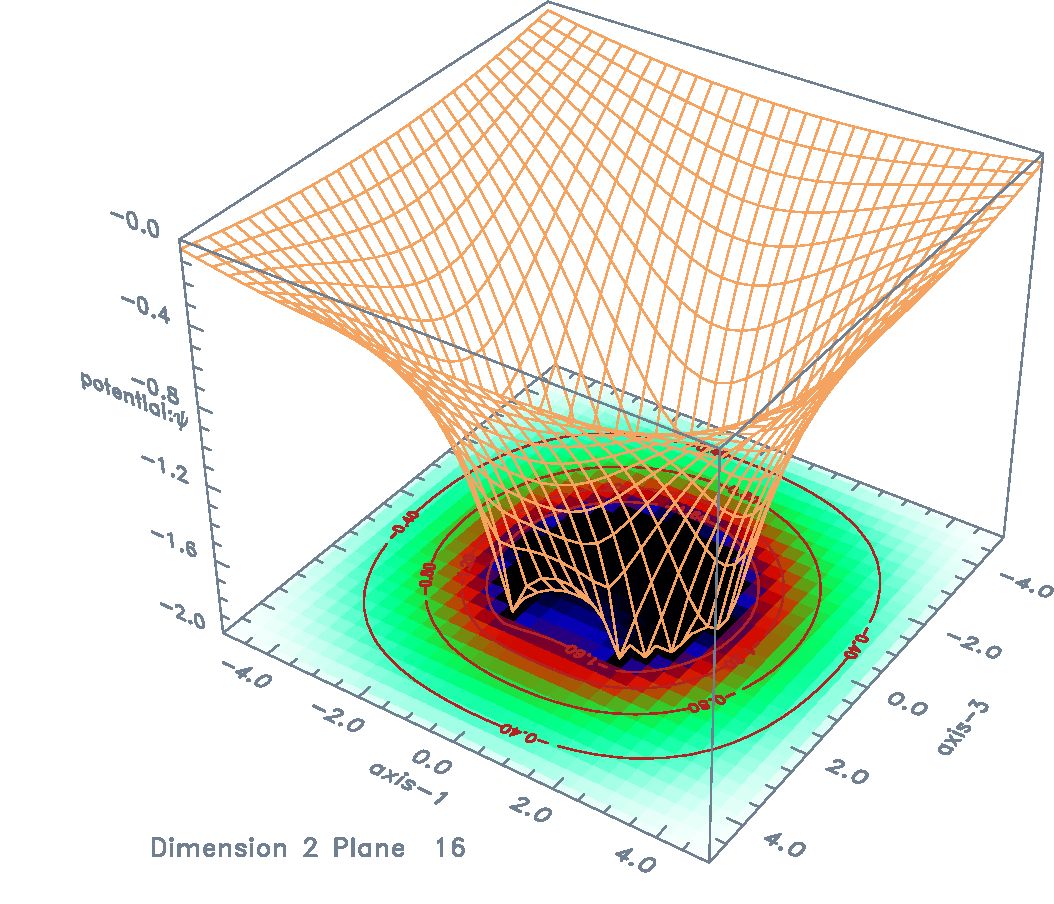
\includegraphics[width=\linewidth]{subtract}\hskip -1cm (c)
\end{minipage}
\caption{Illustration of the subtraction of a cylinder extending to
  half the $32\times32$ domain from a centered sphere. The region in
  which each boundary node lies, on a plane slice through the domain,
  is indicated by an integer consisting of the bits set for each
  object it is inside: 3 means inside 1 and 2. (a) is subtraction 89
  leaving a hollow sphere and (b) is subtraction 88 leaving a solid
  sphere with a cylindrical hole. The parts of the cylinder surfaces
  that are outside the sphere do not create boundary nodes. In (c) is a
  rendering of the potential when charge density in
  negligible, as rendered by COPTIC using the switch -gt.\label{textgraph}}
\end{figure}

The difference between \verb!otype! 88 and 89 is that 88 adds what we
call ``subtractive'' surfaces, while 89 does not, as illustrated in
Fig.\ \ref{textgraph}. Subtracting 89 an
object with null boundary conditions (all zeroes) simply removes the
part of the additive object that lies inside the subtracted
object. What is left is a hollow thin shell of the additive object's
surface with one or two holes in it. [Subtracting 89 a non-null object
adds all of its boundaries everywhere, which is unlikely to be
wanted.]  Subtracting 88 an object removes all the parts of the
additive object within the subtracted, and also adds all the bounding
surfaces of the subtracted that lie inside the additive object. As a
result, new subtractive surfaces of the object appear where its inside
has been removed. It has become a solid object with removed parts
whose inner surfaces are those of the subtracted object. If the
subtracted object has non-null BCs, then those BCs apply to the new
subtractive boundaries. They may therefore be different from the BCs
of the rest of the additive object. If the subtracted object has null
BCs, then it inherits the BCs of the additive object instead. Then the
new subtractive boundaries have the same BCs as the rest of the
resultant object.


No facility (yet) exists for subtracting an object from the
\emph{complement} of another, i.e.\ for subtracting from a negative
object. Generally, adding objects achieves nearly the same result from
the viewpoint of the complementary region. The complementary region is
usually what we care most about.

Subtraction specifications do not increase the object count
\verb!ngeomobj!. Compound objects generated by subtraction cannot be
subtracted from others.

\subsection{Mesh Geometry}

The setting of the mesh spacing in each dimension is specified by
special object lines that may appear anywhere within the object file,
for which \verb!otype! is equal to 91, 92, or 93, referring to the
three directions 1, 2, 3 or x, y, z. The last such line overrules any
earlier lines of the same \verb!otype!. These lines do not constitute
actual objects and do not contribute to the object count
\verb!ngeomobj!.

The format of these special mesh lines consists of a monotonic
sequence of positive integers starting with 1, a separator 0, and then
an equal-length monotonic sequence of reals. This format is thus
$9d,im_1,im_2,...,im_N,0,xm_1,xm_2,...,xm_N$, where $d$ is 1, 2, or 3,
and $N$ is the sequence length. The integer sequence refers to the
mesh index in this dimension, and the real sequence specifies the
position in calculation space of the corresponding mesh node. Between
two indices adjacent in the sequence, the mesh positions are equally
spaced. An example might be
\begin{verbatim}
   92,1,12,21,32,0, -5.,-1.,1.,5.
\end{verbatim}
This line (92) refers to the $y$-direction. It specifies four integers
and four reals separated by 0. The first mesh node (1) is at position
$y=-5$. The twelfth node (12) is at $y=-1$; node (21) is at $y=1$ and the
last node position (32) is at $y=5$. This is therefore a mesh with 32
nodes in the $y$-direction covering the domain $-5$ to $5$, with 11
equal spaces between $-5$ and $-1$, 9 spaces between $-1$ and $+1$,
and 11 spaces between $+1$ and $+5$. The total mesh node-count of each
dimension (32 here) cannot exceed the storage allocated by parameters
\verb!na_i,j,k! in \verb!griddecl.f!. The maximum sequence length that
can be used is specified by parameter \verb!nspec_mesh! in
\verb!meshcom.f!.

Any dimension which is not referred to by a mesh line in the object
file acquires the default specification which is equivalent to
\begin{verbatim}
  9d,1,32,0,-5.,5.
\end{verbatim}
a uniformly spaced mesh of 32 nodes from $-5$ to $5$.

\subsection{Face Boundary Conditions}

Lines in the geometry file can be used to specify the potential
boundary conditions on the rectangular faces of the computational
domain (not specific objects). If \emph{any} face conditions are used,
here or on the command line, then \emph{all} faces use the rectangular
conditions.  Robin boundary conditions, referring to the outward
normal ${\bf n}$ are used in the form
$$A\phi + B \hat{\bf n}.\nabla\phi + C =0$$
The line consists of a type equal to 100 plus the face number,
followed by (up to) 6 reals specifying $A,B,C0,Cx,Cy,Cz$.
The line to set face 2, which is the lower face in the 2-direction, to
have $A=3$, $B=4$, $C=5+6x+7y+8z$ is
\begin{verbatim}
102,3.,4.,5.,6.,7.,8.
\end{verbatim}
The lower faces are 1,2,3; the upper boundary faces are 4,5,6 along
the directions x,y,z.

\paragraph{Periodic potential boundary conditions}
on the faces perpendicular to a particular dimension can be set by a
line in the geometry file. Such lines consist of a single type value lying
between \verb!111! and \verb!110+ndims!. For example
\begin{verbatim}
113
\end{verbatim}
toggles on or off periodicity in the dimension
\verb!type-110=3!. Naturally this sets the boundary conditions for
both lower and upper boundaries. 

When the potential boundary condition is periodic in a certain
dimension, the position of the boundary, or periodic join, of the
computational domain is half way between the boundary node and its
adjacent node within the mesh. In other words, a face node has the
same potential as the node adjacent to the opposite face, because they
are effectively the same place. An adjacent node acquires the charge
contributions of the opposite face node. Face node potentials are
never solved for by the Poisson solver. They are set by the boundary
conditions. Face node charges are never used by the solver, but when
the potential is periodic, they are passed to the opposite adjacent
node. Particles leave the mesh for non-periodic-potential boundaries
when they pass beyond the face node. For a periodic boundary, they
leave when they pass beyond the periodic join.

Any face that is not somewhere explicitly set defaults to the
condition $\phi=0$ if Face Boundary conditions are active.

\paragraph{Periodicity of the computational domain for
  particles}\label{partperiod} can
also be set with the special object \verb!98!, in the form of a line
such as
\begin{verbatim}
98,4,0,0
\end{verbatim} which is equivalent to the switch \verb!-pp4,0,0!.
Each non-zero value sets particle face behavior in that dimension as follows.

\begin{description}
\item[0]  indicates open; particles leave the mesh and others may be
reinjected on the faces. This is the default. 
\item[1] lower absorbing; the lower face in this dimension permits particles
to leave the mesh, but none are reinjected there.
\item[2] upper absorbing; the upper face in this dimension is absorbing;
lower refers to the first value of a mesh specification, and upper the
last.
\item[3] both faces absorb.
\item[4] periodic; particles leaving through one face reappear immediately in the
corresponding position adjacent to the opposite face. They have the same
properties (e.g. velocity) they left with.
\end{description}

Use of boundary-setting lines like these in the object file
\emph{is over-ridden} by any values set by command-line switches.



\subsection{Boolean Region}

An object line of type 99 defines the particle region, the region
inside which the ions are allowed to move, and outside which they are
considered to have escaped, and require reinjection. This line defines
a boolean region, meaning that different objects can be combined by
the operations of AND, OR, or NOT. This provides the ability to define
a complicated volume region in a relatively small number of operations
with respect to various geometrical shapes. The format of this line,
following its type specification (99) consists of successive blocks of
an integer $n_k$ followed by $n_k$ integer values. So a line is
schematically
$99,n1,v_{11},v_{12},...,v_{1,n1},n2,v_{21},v_{22},...,v_{2,n2},...$
The values $v$ refer to actual objects in the object file in the order
in which they appear. (Mesh, subtraction, boundary setting, and boolean lines do
not count as objects but objects of whatever shape, even if their ABC
values are all zero, do.)  The values $v$ may be positive referring to
\emph{inside} or negative referring to \emph{outside}. The list of
blocks is terminated by a zero. All objects in each block are ORed
together. Then the blocks are ANDed. For example
\begin{verbatim}
#     n1 v11 v12  v13 n2  v21  termination
  99, 3, 3,   4,  -6,  1, -5,    0
\end{verbatim}
means that the particle region is (inside 3 OR inside 4 OR outside 6)
AND (outside 5). OR indicates the union of two regions, while AND defines
their intersection. Another example, if we had nested objects with 1
inside 2, and the particles exist between them, is
\verb!99,1,-1,1,2,0!, which illustrates that ``subtraction'' of
objects can be implemented by intersection of the complement.  The
default boolean (if no boolean line is in the object file) is that the
particle region is everywhere within the mesh.


\subsection{Nonuniform Background}

The subtraction of background charge assumed to be attributable to
another species can be chosen in special cases to be non-uniform. 
The non-uniformity is specified by an object file line like this
for example
\begin{verbatim}
# Direction1, 3 terms, coefs 1-3 
   121,         3,     0., 0. ,0.1e-4
\end{verbatim}
The generic form is 
\begin{verbatim}
   12d, Nterms, C1, C2, ..., CNterms
\end{verbatim}
and nonuniformity is permitted in all three directions, each specified
by a polynomial $p_{id}=c_1+c_2x_{id}+c_3x_{id}^2+\dots$ whose
coefficients are read from this line. The coefficients for direction
\verb!id! are stored in an array \verb!bga(i,id)!. Actually the
coefficient C1 is currently irrelevant, because it is overruled by a
calculation that insists that $\int p_{id} dx_{id}=0$, i.e.\ that the
mean nonuniformity in each direction is zero, and adjusts \verb!C1! to
ensure it. As a result, the adjustment, which consists of multiplying
the background by $p_{id}$ (in each specified direction) does not
change the total charge in the domain (if it is empty of objects). If
just the third coefficient is set, then the nonuniformity is
parabolic and the variation term can be considered to be $x^2/2x_c^2$
where $x_c=1/\sqrt{2.C3}$.

\subsubsection*{Summary of domain and boundary setting lines}

\par
\begin{tabular}{|l|l|}
\hline
Leading Entry & Meaning\\
\hline
88,89    & Object subtraction.\\
91-93    & Mesh number and spacing.\\
98       & Particle Periodicity.\\
99       & Boolean of particle region.\\
101-106  & Face potential boundary condition.\\
111-113  & Potential periodicity setting.\\
121-123  & Background nonuniformity.\\
\hline
\end{tabular}

\section{Command Line Parameters}\label{cmdline}

Command line values, entered following switches that take an argument
in COPTIC, must always immediately follow the switch that invokes them
\emph{without whitespace in between}. In other words, any numeric
value must be embedded into the switch argument itself, not regarded
as the next argument on the command line.  The default values of
parameters can be checked by \verb!coptic -h! which prints out the
actual value of the parameter at that stage in processing the command
line. But also the values that a particular run is going to have can
be checked by doing a test run with \verb!-h! added at the end of the
command line. The values printed out will document the values the run
will have. Moreover, any values set by the object file will also be
reflected in the print out.

Each line of the object file that starts \verb!Arguments:! (if any)
adds additional command line switches that are parsed \emph{before}
those that actually appear on the command line.  These switches, like
those that actually appear on the command line, override other
settings in the object file (even settings that appear as special
object lines after the line
\verb!Arguments: ...!).

\subsection{Code control parameters}

\subsubsection*{Particle Numbers and Moving}

\paragraph{-ni....} Set number of particles per node. Zero implies
unset. Default 0.
If set non-zero, specifies the exact number of particles per processor
(node) \verb!n_part!. So that the total number of particles is \verb!nproc!$\times$\verb!n_part!. Every time a particle leaves the domain, a new one is
injected. A fixed number of particles is always present.

\paragraph{-rn....} Set the reinjection number for each step, per
node, \verb!ninjcomp!. 
A total of exactly \verb!ninjcomp! particles per processor is injected
at each step. The number of particles in the simulation therefore
might change.

\paragraph{-ri....} Set the rhoinfinity per node, and hence
\verb!ninjcomp!. Default 100. 
The value of -ri is converted into \verb!ninjcomp! by \verb!ninjcalc! during
initialization. The total \verb!rhoinfinity! is \verb!nproc! times the value
specified. This is the equivalent of -rn but expressed more conveniently.

\paragraph{-rx....} 
Set the potential relaxation rate per step, \verb!crelax!. Default 0.
The edge potential phirein is used to set the factor chi, which
adjusts the reinjection rate by the OML factor, and averein which
increments the injection energy. However, the update of phirein is
multiplied at each step by \verb!crelax!. So if \verb!crelax!=1, the update is
immediate, while if \verb!crelax!=0. the update is zero, and chi and averein
remain zero throughout. Generally when simulating large domains in
which the computational boundary is the particle region, one usually
ought to use \verb!-rx0.! Stability generally requires \verb!crelax<Ti!.

\paragraph{-dt....}
 Set the timestep during the main part of the iteration. Default .1

\paragraph{-da.... with postive value}
 Set the timestep acceleration factor during the first part of
 the time duration, bdt. Default 1. The timestep dt is multiplied by a
 factor $max(1.,(bdt-1.)*(maccel-j+2)/(maccel+1.)+1.)$, where
 \verb!maccel=nsteps/3!.  So the timestep ramps down linearly from bdt*dt to
 dt in the first 1/3 of the timesteps.

\paragraph{-da... with negative value} Instead means increase the
boundary total injection rate by a factor
\verb!bdtnow=1.+abs(bdt)*nf_step*dt! where \verb!bdt! is the value
specified. (You can't both use acceleration and ramp the injection rate.)


\paragraph{-ds....}
Set the particle-advance subcycling. Default 0.  If non-zero, sets the
maximum permissible momentum increment per step ($f*dt$) arising from
electric field. If exceeded, divide the timestep $dtc$ for that
particle by two until either $f*dtc<subcycle$ or the total factor is
$2^3$. Take the corresponding number of shorter steps. A charge of
magnitude $\phi_pr_p$ gives rise to $f=\phi_pr_p/r^2$ at distance $r$,
so subcycling occurs for $r^2<\phi_pr_pdt/subcycle$.

\paragraph{-dd....}
Set the momentum increment, $f*dtc$, value (default 10) above which a
particle is deemed to have encountered a charge singularity and is
dropped from the simulation.

\paragraph{-s....}
Set the total number of steps to take. Default 5. 
If restarting, this is the number of \emph{additional} steps. 

\subsubsection*{Plasma Parameters}

\paragraph{-t....}  Set the (ion) temperature, $T_i$ ($/T_e$). Default 1.

\paragraph{-tp....} Set perpendicular (to B) temperature. Default
$T_i$. [A subsequent -t switch will override this setting.]

\paragraph{-l....}  Set the electron Debye length, \verb!debyelen!. Default 1.

\paragraph{-v....}  Set the drift velocity, \verb!vd!, of the background ions . Default 0.

\paragraph{-vx -vy -vz...} Set the direction cosines of the drift
velocity, not necessarily normalized. Default (0,0,1).

\paragraph{-tge...} Set the reference position and gradient of
$T_e$. Six reals must follow the switch without spaces. The first
three are the coordinates of the reference point at which $T_e=1$ in
normalized units. The second three are the components of the gradient
of $T_e$ (in normalized units). If the gradient is such as to cause
the local $T_e$ to become non-positive anywhere on the grid, a fatal
error will terminate the initialization. Default: zero gradient. 

\paragraph{-ng...} Set the external gradient of $n_e$. Three reals
must follow the switch without spaces. They are the inverse
scale-lengths (logarithmic gradient), in the three coordinate
directions, of the density. The scale lengths, that is the
logarithmic gradients, are uniform throughout the domain. The center,
where the density is equal to one, is at the reference point defined
by any -tge call, (or otherwise at 0,0,0). The default density gradient is zero. There can be
no density gradient parallel to the magnetic field or if there is no
magnetic field.

\paragraph{-sp} Add a particle species. Thereafter particle parameters
refer to the new species. Normally the second species is electrons.

\paragraph{-zm...} Set the charge-to-mass ratio. Default 1 ions -1836
electrons.

\paragraph{-nr...} Set the number-ratio of the ions to the current
species. By default this is equal to 1. Other choices are
possible. For example using square root of the inverse mass ratio
makes the step length of particles of equal temperatures equal. The
number of steps of this species per ion step is equal to the
number-ratio, so the number of depositions of electrons and ions is
equal (for the background).  Setting -nr1 uses equal numbers of
particles and no substepping.

\paragraph{-sb...} Set Boltzmann fraction $f_b$
(\verb!boltzamp!). When both electrons and ions are being modelled as
particles (more than one particle species is present) this switch
should occur \emph{after} the -sp switch [because -sp reinitializes
\verb!boltzamp! to zero.] It is physically equivalent
to adding an additional species whose density is equal to
$f_b\exp(e\phi/T_e)$. That is, like Boltzmann electrons.  It is
implemented through the function \verb!faddcomp!. The charge of
particle-species 2 is reduced by the factor \verb!1-boltzamp!, which
is the fraction of that species (by default electrons) represented by
particles, but their number density remains the same as species 1.  The
addition helps to stabilize long-wave-length fluctuations in regions
that are much larger than the Debye length. The fraction required is
of order the ratio of the Debye length to the domain size, when this
is small. If either there is more than one species or \verb!holepsi!
is non-zero (switch \verb!-ih! is set nonzero), then \verb!boltzamp!
is ramped down to zero in the first third of the timesteps.

\paragraph{-sb0} When only one species is present, the switch usage
-sb0, setting \verb!boltzamp! to zero, removes the effective Boltzmann
response from the calculation and \emph{instead} adds a uniform
negative background charge.  This is physically equivalent to ions
moving in an immobile (uniform) electron background.  COPTIC then runs
as a true single-species PIC code. Setting a non-zero but non-unity
value of \verb!boltzamp! removes some of the Boltzmann electron
response and adds a consistent fraction \verb!1-boltzamp! of immobile
negative background. More relevantly, the moving particles can then be
considered to be electrons in a uniform ion background, (but with
reversed charge signs unless \verb!-zm-1.! is used). Appropriate
stability limits on time-step must be observed as if the times-scales
were electron. Thus one should consider velocities to be normalized to
$\sqrt{T_e/m_e}$. The (electron) plasma frequency in computational
units is then $\omega_{pe}=1/\lambda_{De}$, and stability requires
$\omega_{pe}dt = dt/\lambda_{De}<1$.

\paragraph{-ih[...]} Set parameters of a phase-space hole in particle
initialization for the current species. Only one species can be
initialized as a hole; so this switch overrules and disables hole
settings for any previous species. Up to six parameters are set by
succeeding values separated by commas (no spaces). The parameters and
their defaults are \verb!holepsi! [0.1] the hole (peak) potential,
\verb!holeum! [0.]\ the speed of the hole relative to the mean of the
untrapped Maxwellian distribution, \verb!holelen! [4.]\ the length of
the hole in Debye lengths, \verb!holeeta! [2.]\ the power that
determines the hole shape (2 is a parabola), \verb!holepow! [0.5]
which governs the interpolation power when the hole transverse trapped
temperature is other than the external, and \verb!holerad! [0.] the
radius of the hole in the transverse plane.  The spatial direction of
the velocity trapping of the hole must be one of the axes, and is
determined by the B-field direction (unless it is not axis-aligned, in
which case axis 1 is chosen). When plasma drift is present, its
component in the trapping direction is added to \verb!holeum! to give
the net hole speed relative to the mesh; so setting \verb!holeum! equal to
minus the drift gives a hole stationary in the mesh.  In the other directions
uniform Maxwellian initialization is used. A hole is incompatible with
non-zero collisions. Single-species holes typically use \verb!-sb0!
(or small), a uniform neutralizing background. Then \verb!-zm-1!,
negative charge particles means the particles can be considered to be
electrons and the velocity units $\sqrt{T_e/m_e}$ (assuming $T=1$).

\paragraph{-pi...} Use quiet particle initialization. Reads an integer
argument from the switch, which gives the maximum number of qblocks in
each dimension, and if greater than zero causes the qinit code (rather
than the defaults pinit or trapinit) to be used for particle
initialization. If no argument can be read, then the number of qblocks
is set to a default of 30.



\subsubsection*{Neutrals, Collisions, Magnetic Field}

\paragraph{-ct....} Set the collision time, colntime. Default 0 [off].

\paragraph{-vn....} Set the neutral drift velocity, \verb!Vneutral!. Default \verb!vd!.

\paragraph{-tn....} Set neutral temperature. Default \verb!Ti!. 

\paragraph{-Ef....} Set the fraction of the relative drift between
background ions and neutrals (vd-vn) that is driven by an external
electric field Eneutral not expressed as the gradient of phi.

\paragraph{-cp....} Set the power of (total) speed that the
collision frequency is proportional to. Thus \verb!-cp0.! is constant
collision frequency and \verb!-cp1.! is constant cross-section. The
thermal spread of the neutrals is only approximately accounted for in
using this collision setting.


\paragraph{-Bx.. -By.. -Bz..} Set the respective components of the
magnetic field. 

\subsubsection*{Diagnostics and Averaging}

\paragraph{-w....}  Set period of write steps. Default 99999=never.
This says how often (in steps) the total particle data is written out to
disk. It is independent of the diagnostic averaging or moment writing.
The data overwrites the files of prior steps, giving the running
values. In any case, the particle flux data for all steps is contained in
the files. If the write step period is set to a negative number, then
only the particles from node 0 (the master) are ever
written to disk. 

\paragraph{-a....}  Set the averaging time, \verb!iavesteps!. Default 100.
This controls the number of steps over which diagnostic and other
quantities are averaged. Writing or plotting of diagnostic and
distribution data takes place only every \verb!iavesteps! steps.

\paragraph{-pd...}
Set distribution diagnostics. Bit1: write, Bit2: plot. Default 0.
This controls whether particle distribution diagnostics will be
written and/or plotted at the end of each \verb!iavesteps! steps. 

\paragraph{-pu...}
Set the particle distribution diagnostics to \verb!nsbins! uniform
bins in each velocity direction. [Without this setting, importance
sampling sets non-uniform bins.] This setting also turns on
accumulation of 2-D distributions; so the pex files will be larger.
Does nothing if \verb!-pd! is unset.

\paragraph{-md....}  Set number of diagnostic moments to save (max 7). Default 0.
This controls which diagnostic files and messages will be written
every istepsave steps. If zero, no files or messages.

\subsubsection*{Boundary Conditions}

\paragraph{-bc....} Set the type of boundary conditions. (This is
superceded and disabled by the -bf/-bp type below if present.) The single
integer parameter's bits are interpreted as follows.  Bit 1 Mach
cylinder (if set) else spherical logarithmic gradient.  Bits 2-7 set
face to zero (only 3 implemented). Bits 8-13 set corresponding face to
have ``second derivative'' boundary condition (only 13 implemented).

\paragraph{-bf....} Set the face boundary conditions. (Superceded by
-bp type below if present.) This command requires multiple additional
arguments separated by commas but no spaces. Its form is
\verb!-bfid,AF,BF,C0F[,CxF,CyF,CzF]!. Here \verb!id! is the face
number (1-3 lower, 4-6 upper, 7 set all faces, 0 reset all), AF, BF,
C0F, are the Robin condition coefficients referring to the outward
normal potential gradient. But if present then CxF, CyF, CzF are the
gradients of the C-coefficient of the Robin condition, so that
C=C0F+CxF.x+CyF.y+CzF.z . If the Robin B-value, BF, is equal to zero,
then assume AF is equal to 1; so -C is the set value of $\phi$.

\paragraph{-bp....} Choose the dimension indicated by the single
integer parameter. Toggle on (or off) periodic boundary conditions on
potential for that dimension. Implies using the rectangular -bf
overall scheme if periodicity is on, but overrides the behavior in the
chosen dimension.

\paragraph{-pp....} Set the values of the particle ``periodicity'' at
the domain boundary for three dimensions, for example \verb!-pp2,4,4!.
The behaviour for each dimension is 0: open boundary; 1: lower
boundary absorbing; 2: upper boundary absorbing; 3: both faces absorb;
4: particles that leave the mesh are relocated at the corresponding
periodic position within the mesh, rather than reinjected. See
\ref{partperiod}.

\subsubsection*{MPI, Restart, and Files}

\paragraph{-id....} Set the number of MPI blocks in each
dimension. For example, \verb!-id2,2,8! would prescribe an MPI
cartesian block array of $2\times2\times8$ (in the dimensions $xyz$).
The total number of blocks (32 in this case) must be equal to the
number of MPI processes on which coptic is running. If it is not, then
the switch has no effect, and the MPI cartesian topology is decided
automatically, as it is normally by default.

\paragraph{-ofFilename} Set the name [including path] of the object
file. Default ccpicgeom.dat

\paragraph{-fs....}  Attempt to restart the code from a saved
state. The integer switch indicates 0: no restart; bit-1 set [1]: read
the particle files so as to initialize, and start the step count at 1;
bit-2 set [2 or usually 3]: read the flux file and particle and
potential and start at the next step after the prior run. Normal full
restart is -fs3. If bit-3 set [4]: then use the basename
``restartfile'' for the files from which to restart.

\paragraph{-fn....} Set the path where particle files are read from
and written to.

\subsection{Display and debugging parameters}

Although COPTIC gives no graphic output unless explicit switches are
set, it can give a variety of diagnostic information during its
operation, including sophisticated multidimensional plots of current
mesh parameters.  The graphics output will generally work only on
builds that include X libraries (see section \ref{building}). One
ought not otherwise to use the display switches.

\begin{verbatim}
Debugging switches for testing
 -gt   Plot regions and solution tests.
 -gi   Plot injection accumulated diagnostics.
 -gn   Plot collisional reinjection distribution.
 -gg   Run continuously without pausing.
 -gp -gd[] Plot slices of setup; plus potential, density. [At step n]. [    1
 -gf   set quantity plotted for flux evolution and final distribution. [   -1
 -gw   set objplot sw. [+256:intercepts] Shade by 1:flux 2:flux-density[    1
 To plot intersections with objects use -gf and -gw
 -gc   set wireframe [& stencils(-)] mask. objects<->bits. [    0
 -gr   set override view scale (box size) for -gc, -gf plots.  [   0.000
 -go   set No of orbits(to plot on objects set by -gc). [    0
 -at   set test angle. -an   set No of angles. 
 -ck   set checking timestep No. [    0
 -h -?   Print usage.
 -hg     Print debugging/plotting switch usage.
 -ho     Print geomobj file format description
\end{verbatim}
These are required only for rather sophisticated use of COPTIC, and
should be understood by reference to the source and comments. In
brief, \verb!-gt! gives text representations of region and volumes
slices and does plots of slices through the mesh of the disallowed
particle region and the test initial potential solve. See Fig.\
\ref{textgraph}. It is helpful for visualizing the mesh and the areas
affected by objects. \verb!-gi! is for debugging
reinjection. \verb!-gp! and \verb!-gd! cause plotting slices of
potential and density at an optionally specified step interval, which
can be useful to verify both the grid and the initial evolution of the
parameters. Their displays are similar to Fig.\ \ref{textgraph}(c),
and all allow navigating to different slices, rotating the view and
detailed inspection. \verb!-gc! sets through its bits the objects to
display in wire-frame fashion initially (so -gc1023 displays the first
9 objects). It can be useful (possibly in combination with \verb!-gr!) to
visualize the representation of objects near the origin. See Fig.\
\ref{manyobj}. 
\begin{figure}[htp]
  \centering
  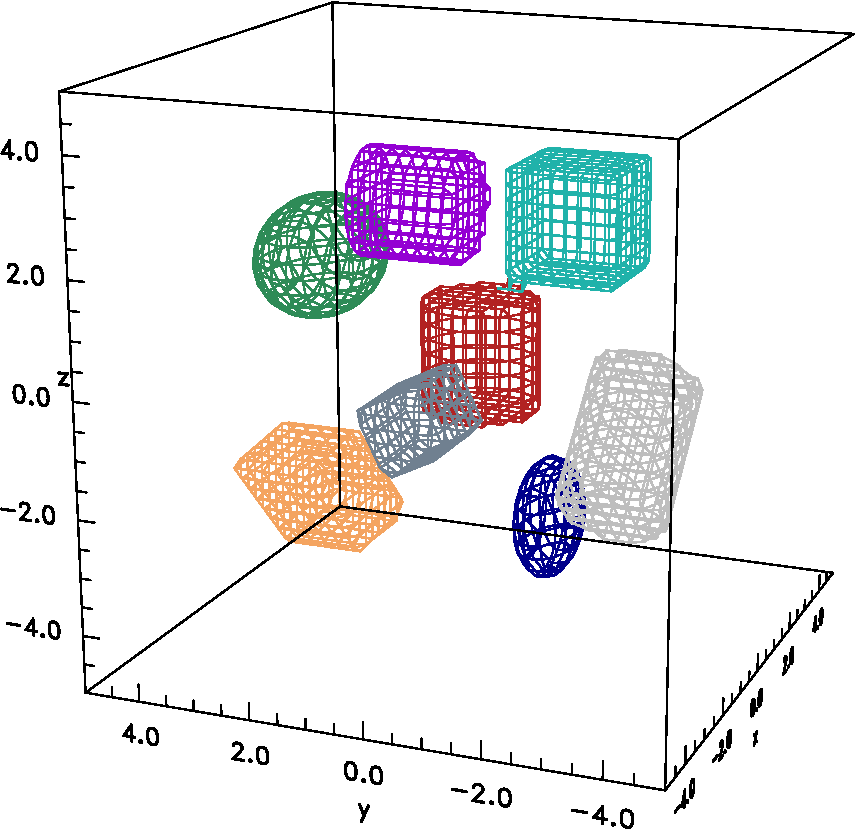
\includegraphics[width=3in]{manyobj}
  \caption{Rendering of a 3-D view of a case with numerous objects of
    different types using switch -gc.\label{manyobj}}
\end{figure}

\verb!-gf!  sets the flux quantity to be plotted in 3-D graphics
emitted after the final step. Objects that do not have flux collection
turned on are displayed with their faces colored simply to
differentiate them. Fig.\ \ref{manyflux} illustrates this. \verb!-gw! specifies non-standard switch settings
to the \verb!-gf! plots.
\begin{figure}[htp]
  \centering
  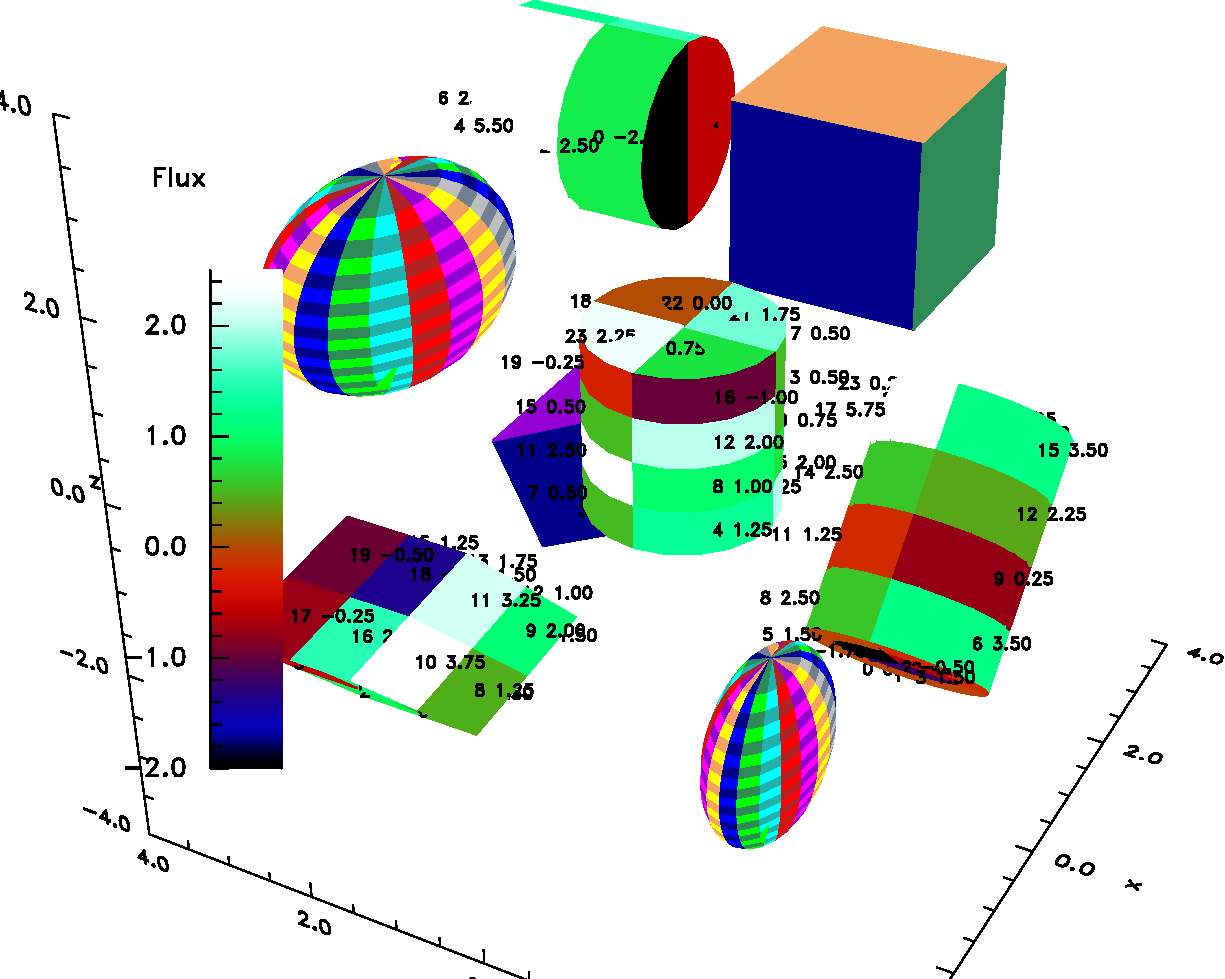
\includegraphics[width=4in]{manyflux}
  \caption{Rendering of the fluxes to faces of different objects using
    switch -gf.\label{manyflux}}
\end{figure}


\section{Data Structures}

This section of the manual contains code segments that might not be
fully up to date, so the reader should defer to source if
discrepancies are present. It is intended to help understand the code
for purposes of code development.

\subsection{Dimension}

Is set by including file \verb!ndimsdecl.f! which defines the
parameters \verb!ndims!, \verb!ndimsmax!, and \verb!nspeciesmax!.


\subsection{Particles}

Particle information resides, as defined in file \verb!partcom.f!, in
common block \verb!particles!.
\begin{verbatim}
      integer nparta(nspeciesmax)
c Maximum particle slot that we must examine
      integer iocparta(nspeciesmax)
c Starting particle slot
      integer iicparta(nspeciesmax+1)
c Particle position and velocity (3D cartesian) in the order:
c (x,y,z) (vx,vy,vz) (xm,ym,zm) where xm... is the mesh position.
      real x_part(idtp,n_partmax)
c Ratio of the number of steps and inverse number of particles:
      integer numratioa(nspeciesmax)
c Timestep (unperturbed).
      real dt
c Control of diagnostics
      logical ldiags
c Rho at infinity totalled over processes
      real rhoinf
c Number of reinjections this step
      integer nrein
c Average potential of reinjections
      real phirein
c Number of independent processors
      integer numprocs
c Number of reinjections at each step (if non-zero)
      integer ninjcompa(nspeciesmax)
c Rho at infinity per processor, relevant only in setup.
      real ripernode
c Factor by which we relax the rhoinf calculation. 1 immediate, 0 never.
      real crelax,caverein,chi
c Flags for which dimensions are periodic or absorbing for particles.
c 0 open, 1 lower absorbs, 2 upper absorbs, 3 both absorb, 4 periodic
      integer ipartperiod(ndims)
c Effective face area for purposes of reinjection. Small if periodic.
      real fcarea(ndims)
c Whether not all directions of particles are periodic
      logical lnotallp
      integer n_part,iic_part,ioc_part,ninjcomp
      equivalence (n_part,nparta(1)),(iic_part,iicparta(1))
     $     ,(ioc_part,iocparta(1)),(ninjcomp,ninjcompa(1))
      common/particles/x_part,nspecies
     $     ,nparta,iicparta,iocparta,ninjcompa,numratioa
     $     ,dt,ldiags,rhoinf,nrein,phirein,numprocs
     $     ,ripernode,crelax,ipartperiod,fcarea,lnotallp
     $     ,caverein,chi
\end{verbatim}
The number of active species is \verb!nspecies!.
The number of active particles of each species is
\verb!nparta(ispecies)!. Each species occupies particle slots starting
at \verb!iicparta! and the maximum slot in the particle array that
might have a particle in it is \verb!iocparta!. The last species must
not go past the allocated length of the particle array
\verb!n_partmax!. The ion density at infinity summed over the
\verb!numprocs! processes is \verb!rhoinf!. Equivalences to the
standard single particle species parameters assist with legacy code
and clarity. The number of reinjections
in this step is \verb!nrein!  and the average potential at which they
were reinjected is \verb!phirein!. If \verb!ninjcomp! is non-zero,
then it defines the specified number of reinjections per step. [But is
that changed during acceleration?]  The other scalar variables
describe a few other setting such as the unperturbed timestep
\verb!dt!.

The main data consists of \verb!x_part! whose first index references
the {\bf position}, {\bf velocity}, and {\bf fractional mesh
  position}. The flag \verb!if_part! indicates whether there is actually
a particle in this storage slot, and \verb!dtprec! saves the size of
the previous timestep this particle executed.

The file \verb!partcom.f! also defines the storage space for tracking
orbits of up to \verb!nobsmax! particles for up to \verb!nstepmax! steps.
\begin{verbatim}
        real xorbit(nstepmax,nobsmax),yorbit(nstepmax,nobsmax),
     $     zorbit(nstepmax,nobsmax)
      integer iorbitlen(nobsmax)
      common /orbits/norbits,iorbitlen,xorbit,yorbit,zorbit
\end{verbatim}


\subsection{Fields}

Potentials, charges and fields are defined on a cartesian mesh. It is
described by two commons in \verb!meshcom.f!. The first is the mesh
specification data \verb!/meshspec/! that is read in from the object file.
It is used in the routine \verb!meshconstruct! to construct the mesh,
but is generally unimportant during running, because the information
is coded into the second common \verb!/sormesh/!.
\verbatiminput{../src/meshcom.f} 

The array \verb!xn! contains the x, y, and z mesh positions
concatenated one after the other. Its allocated length,
\verb!ixnlength! must exceed the sum of the mesh numbers for the three
dimensions. It is usually indexed using a mesh pointer
\verb!ixnp(ndims_mesh+1)! whose integer values are the offsets from
the start of array \verb!xn! at which each new dimension's mesh
positions begin. Therefore \verb!ixnp(1)=0!; and \verb!ixnp(id)+1! is
the index in \verb!xn! of the start of the coordinate values of mesh nodes
for dimension \verb!id!. The final value, \verb!ixnp(ndims_mesh+1)!
points to the address of the last of the last-dimension's
positions. Therefore for each dimension \verb!id!, the mesh ranges
from \verb!xn(ixnp(id)+1)!  to \verb!xn(ixnp(id+1))!  and the length
of the mesh is \verb!ixnp(id+1)-ixnp(id)!.

\paragraph{Non-standard stencils,} which occur at object surfaces,
are controlled by data structures in file \verb!objcom.f!. 
\verbatiminput{../src/objcom.f}
The array \verb!dob_cij! which is equivalenced to \verb!idob_cij!
contains the information accessed by a pointer into its second index.
For any node of the mesh, there is a pointer which if non-zero refers
to the corresponding column of this array. The integer
\verb!oi_cij! is the column last filled with data. 

Each column of \verb!dob_cij! contains data describing the stencil
surrounding this boundary node. The fractional nodal distance to the
adjacent node (equal to 1 if there's no interface in this direction), and the
values of $B/A$ and $C/A$ are stored for the forward and backward
directions of each coordinate. 

Then come the diagonal coefficient, boundary potential contributors,
and the following integers: the flags, the region-code of this point,
the inverse pointer back to the node within \verb!cij(2,2,2)!, the
intersection object code, and finally an extra pointer which if non
zero points to a different column of \verb!dob_cij! used to chain
extra data specifically for a boundary whose potential varies with
time (because it is floating or insulating). The extra data consists
for each stencil direction of the triple: \verb!iobj! which references a
flux-collecting object number, \verb!ijbin!, the flux facet on that
object which this stencil intersects, and \verb!coefoa!, the value by
which to multiply $C$ when adding it to the boundary contribution.


\paragraph{The field arrays} are declared in the main program in \verb!coptic.f!,
not in common, using length parameters defined in file \verb!griddecl.f!.
\begin{verbatim}
      real u(na_i,na_j,na_k),q(na_i,na_j,na_k)
      real qave(na_i,na_j,na_k),uave(na_i,na_j,na_k)
      real psum(na_i,na_j,na_k),volumes(na_i,na_j,na_k)
      real cij(2*ndims_cij+1,na_i,na_j,na_k)
\end{verbatim}
The potential and charge are \verb!u, q!. The volumes of the cells
whose centers are at the nodes are calculated once using routines from
\verb!volint.f! and stored in \verb!volumes!. The allocation sizes can
convenently be adjusted using the script \verb!setdimens!

The stencil information is calculated by \verb!cijroutine! and stored
in \verb!cij!. Its first index references the stencil coefficients in
the directions $\pm x, \pm y, \pm z$, followed by a single value
which, if non-zero, is a pointer to the second index of \verb!dob_cij!
and indicates that this is a non-standard stencil needing special
interpretation. The maximum length \verb!Lobjmax! is therefore limited
to the largest integer that can be correctly represented by a
real. Since only boundary nodes have non-zero pointers, this is not a
severe limitation, and it could be fixed by equivalencing cij to an
integer array.

\subsection{Collisions}

Collisions with neutrals are governed by a collision time
\verb!colntime! which if zero means there are no collisions.
\verbatiminput{../src/colncom.f}

The collision frequency is by default independent of particle
velocity. However, if \verb!colpow! is non-zero, then the collision
frequency is taken to be \verb!((Tneutral+v2)/Ti)**(colpow/2.)! times
\verb!colntime!, where \verb!v2! is the square of the particle
velocity. Thus \verb!colpow! is the power of the velocity to which the
collision frequency is proportional, except that the collision
frequency does not go to zero at zero ion velocity, because of the
background velocity of the neutrals. This approximates a cross-section
that is proportional to velocity to the power \verb!colpow-1!.

When the background neutral velocity, \verb!vneutral!, is not equal to
the background ion drift velocity, \verb!vd!, then some field must
drive \verb!vd!. A fraction \verb!Enfrac! is driven by a field
\verb!Eneutral! which is a background force field not accounted for by
the gradient of the potential $\phi$. The rest is supposed to be
driven by $-\nabla\phi$.

\subsection{Objects}

The parameters of the objects are maintained in a common within file
\verb!3dcom.f!. Parameters define the relevant array sizes and provide
pointers to the positions of different values within the array
\verb!obj_geom!, which contains most of the data.

\begin{verbatim}
      parameter (ngeomobjmax=31)
      parameter (otype=1,oabc=2,ocenter=5,oradius=8,ocylaxis=11)
      parameter (ovec=oradius,ocontra=oradius+9,ocylrad=oradius+6)
      parameter (ofluxtype=ocontra+9)
      parameter (ofn1=ofluxtype+1,ofn2=ofluxtype+2,ofn3=ofluxtype+3)
      parameter (omag=ofluxtype+1,offc=ofluxtype+4)
      parameter (ocgrad=offc+1,obgrad=ocgrad+3,oagrad=obgrad+3)
      parameter (odata=oagrad+2)
      real obj_geom(odata,ngeomobjmax)
\end{verbatim}
The data positions in the input file for different objects are
specified in Table \ref{geomtable}. The index parameters that refer to
the positions are indicated in the first column. Each line in the
table refers to multiple numbers that are read into storage positions
indicated by integer positions following the parameters. Parameters
refer to the first position of a range.  Integers in parentheses refer
to storage positions that are not line entry positions. Surfaces of
revolution are expressed in terms of $r,z$ pairs in fractions of the
reference radius and the reference $z$-length (from the base to the
apex).
\begin{table}[htp]
\caption{Position of geometric data in object file for different objects.\label{geomtable}}
\begin{tabular}{|l|l|l|l|l|l|}
\hline
  Byte-1: & 1& 2& 3& 4& 5\\
  Object: & Spheroid& Cuboid& Cylinder& Parallelopiped& General
  Cylinder\\
\hline
\verb!oabc! 2-4 & ABC  & ABC  & ABC  & ABC  & ABC 
\\
\verb!ocenter! 5-7 & Center& Center& Center& Center& Center\\
\verb!oradius! 8-10 & Radii& ${1\over2}$-Sides&
Radii&  vector-1& Axis-${1\over2}$-vector\\
\verb!ocylaxis! 11-16 & & & Axis number& vector-2,3& Ref-vector, radius\\ 
\hline
\end{tabular}

\begin{tabular}{|l|l|}
\hline
  Byte-1: & 6 or 7 \\
  Object: & Surface-of-Revolution\\ 
\hline
\verb!oabc! 2-4 & ABC  \\
\verb!obase! 5-7 & Base\\
\verb!oapex! 8-10 & Apex\\
\verb!ocylaxis! 11-13 & Reference Vector\\
\verb!ocylrad! 14 & Reference radius\\
\verb!onpair! (27) & Number of $rz$-pairs \\
\verb!opr+k-1,opz+k-1! & Pair $r_k,z_k,\ k=1,n$ \\
\hline
\verb!ofluxtype! (28) & Number of fluxes \\
\verb!ofn1! (29) &  Number of $\theta$-divisions\\
\verb!opdiv=opr!+2*\verb!ovlen! & Face-divisions $n[+1]$\\
\hline
\end{tabular}
\end{table}

In addition, the flux accumulation number of object \verb!iobj! is
given in \verb!nf_map(iob)!.
\begin{verbatim}
      integer nf_map(ngeomobjmax)
      parameter (ibtotal_part=100)
      integer ibool_part(ibtotal_part)
      integer ifield_mask
      integer iptch_mask
      logical lboundp
      character*50 rjscheme
      common /objgeomcom/ngeomobj,obj_geom,nf_map
     $     ,ibool_part,ifield_mask,iptch_mask,lboundp,rjscheme
\end{verbatim}

The particle region boolean is stored as an integer array. An integer
masks the objects to indicate which have no consequences for the
potential. A point-charge mask indicates which objects are point
charges. A character variable indicates the reinjection scheme. [And
  why is that here?]

\subsection{Flux and Stress}\label{fluxstruct}

\paragraph{The accumulation of flux} to different regions (called facets) of the
surfaces of different objects is performed with data structures
defined in file \verb!3dcom.f! using an explicit heap of data
\verb!ff_data!, into which various addresses and pointers are defined.
\begin{verbatim}
      parameter (nf_posdim=4,nf_ndims=3)
      parameter (nf_quant=5,nf_obj=20,nf_maxsteps=3000)
      real ff_rho(nf_maxsteps),real ff_dt(nf_maxsteps)
      parameter (nf_datasize=10000000)
      parameter (nf_flux=1,nf_gx=2,nf_gy=3,nf_gz=4,nf_heat=5)
      parameter (nf_p1=0,nf_p2=-1,nf_p3=-2,nf_p4=-3)
      parameter (nf_pr=nf_p1,nf_pt=nf_p2,nf_pz=nf_p3,nf_pa=nf_p4)
      integer nf_step,mf_quant(nf_obj),mf_obj
      integer nf_posno(nf_quant,nf_obj)
      integer nf_dimlens(nf_quant,nf_obj,nf_ndims)
      integer nf_faceind(nf_quant,nf_obj,2*nf_ndims)
      integer nf_geommap(nf_obj)
      integer nf_address(nf_quant,nf_obj,1-nf_posdim:nf_maxsteps+2)
      real ff_data(nf_datasize)
      common /fluxdata/nf_step,ff_rho,ff_dt,mf_quant,mf_obj,nf_posno
     $     ,nf_dimlens,nf_faceind,nf_geommap,nf_address,ff_data
\end{verbatim}
Data is acquired for each time step up to the maximum available size
\verb!nf_maxsteps!. For each of up to \verb!nf_obj! objects, we
collect up to \verb!nf_quant! flux quantities, corresponding to
particle flux, three components of momentum flux, and heat flux. The
actual number of quantities tracked for object \verb!i! is
\verb!mf_quant(i)!.  The collection is tracked by the facet into which
the collection occurs. Each object has, for quantity \verb!j! a total
of \verb!nf_posno(j,i)! facets. (At present these are the same for all
\verb!j!.) For different shaped objects, the facet fluxes are
designated by appropriate dimensional arrays, whose dimensional
structure is \verb!nf_dimlens(j,i,k)!, so that total number of facets,
\verb!nf_posno(j,i)! is equal to the product over \verb!k! of the dimlens.
The starting position, within the heap, of the flux data for step \verb!n! is 
\verb!nf_address(j,i,n)!. The offset to the start of the different
faces of a parallelopiped type object are \verb!nf_faceind(j,i,k)!,
where \verb!k! is the face number (up to $2*ndims$).
Because the flux-tracking objects are not all the objects there are,
they are numbered differently from the objects within
\verb!objgeomcom!, and we need mapping back and forth. 
The index within \verb!obj_geom! that
corresponds to this flux-tracked object \verb!i! is
\verb!nf_geommap(i)! (just as \verb!i=nf_map(nf_geommap(i))!.

\paragraph{Stresses} contributing to the forces on objects are
accumulated using integrations over positions numbering \verb!ns_nt! and
\verb!ns_np! in two directions the surface of objects (only
spheres at present). 
\begin{verbatim}
      parameter (ns_ndims=3)
      parameter (ns_nt=20,ns_np=20)
      integer ns_flags(nf_obj)
      real fieldforce(ns_ndims,nf_obj,nf_maxsteps)
      real pressforce(ns_ndims,nf_obj,nf_maxsteps)
      real partforce(ns_ndims,nf_obj,nf_maxsteps)
      real colnforce(ns_ndims,nf_obj,nf_maxsteps)
      real charge_ns(nf_obj,nf_maxsteps)
      real surfobj(2*ns_ndims,ns_nt,ns_np,nf_obj)
      common /stress/ns_flags,surfobj,fieldforce,pressforce
     $     ,partforce,colnforce,charge_ns

\end{verbatim}

\subsection{Diagnostics}

\paragraph{Particle distribution} diagnostics structures are defined in file
\verb!ptaccom.f!, and used only in routines in \verb!partaccum.f!. 

For accumulation of the distribution averaged over large regions, the
structures in common \verb!/cartdiag/! are used.  There are
\verb!nptdiag! points in each direction for position and velocity.
\verbatiminput{../src/ptaccom.f} 
Spatially resolved velocity distributions
are collected over blocks of cells. The number of such blocks is given
by \verb!parameter(nsub_i=15,nsub_j=15,nsub_k=15)!  The velocity bins
are unevenly spaced using an importance algorithm, so as to allow
representation of the velocity distribution with a limited number,
\verb!nsbins!, of bins that are the combination of bins defined over
\verb!nptdiag! velocities in the common \verb!/subdiag/!.  There
\verb!ibinmap! is the map from uniform bins to combined bins;
\verb!vsbin! is the central velocity of the combined bin; \verb!csbin!
is the number of fine bins in the combined bin. The spatially resolved
distribution data is \verb!fvx!. Finer velocity resolution may be
obtained by using larger \verb!nsbins! than the typical (parameter) 32
but storage demands eventually become excessive.  Uniform binning
may be obtained by putting \verb!nptdiag=nsbins!.

\section{Code Execution Flow}

COPTIC is capable of massively parallel calculation using the MPI
libraries for inter-process communication. Each particle is assigned
to a specific processor. So increasing the total number of particles
can be done with hardly any execution time degradation simply by
adding processors. The field-solve work is shared by the processors in
parallel and the resulting field for the whole mesh is communicated to
all processors. The code will run perfectly satisfactorily, however,
on a single processor.

\subsection{Overview of main program}

\paragraph{Parameter Initialization} of a few parameters occurs
first, generally by assignment (rather than data) statements. The MPI
system is initialized by calling \verb!mpigetmyid!, from file
\verb!mpibbdy.f!, which contains the MPI block boundary communications
code. The communicator id, \verb!myid!, of the process is
determined. The master node (or the unique node for serial runs) has
\verb!myid=0!. 

\paragraph{Command line arguments} are dealt with by two calls to
\verb!copticmdline!. The first sets most defaults but returns the name
of the object file, which is then read so that it sets parameters.
The second call to \verb!copticmdline! then iterates through all the
arguments until they are exhausted or an error occurs. In the latter case,
or when it is specifically asked for, a help message is given, which
indicates the current values of the command-line parameters after
which the program then terminates. By this two step process, any
command line argument that sets a parameter \emph{overrides} any
values set by the object file.

\paragraph{Initializations} are performed as follows.
\sentence{The mesh is constructed} \verb!meshconstruct!, and if
necessary for this type of reinjection its geometry is initialized
by \verb!geominit!.

\sentence{Injection is initialized} if we have specified a certain
rho-infinity per node, \verb!ninjcalc!.

\sentence{Flux data collection is initialized} \verb!fluxdatainit!.

\sentence{Stencil data is calculated} by iterating over the mesh the
\verb!cijroutine!. If warnings of object-mesh clashes are received,
then the mesh is shifted slightly and things are reinitialized.

\sentence{Stored volume information} is sought and read using
\verb!stored3geometry!. If appropriate information is not retrieved, then

\sentence{Volumes are calculated}

\sentence{Various cij pointers masks and flags are set}

\paragraph{Optional diagnostic displays} of the solver geometry are given:

\sentence{Optionally, regions and volumes are displayed} using simple text
graphs. 

\sentence{Optionally, cij is plotted} showing intersections of the
lattice with the objects.

\paragraph{Fields and particles are initialized} in appropriate order
as follows.

\sentence{Charges and potentials are zeroed}

\sentence{An initial Poisson solution} is calculated with zero
charge, and optionally tested against vacuum solutions.

\sentence{The Random number generator is initialized} using the (MPI) id
number. 

\sentence{Particles are initialized} randomly.

\sentence{Force tracking is initialized.}

\sentence{Optionally, a restart} is attempted from saved disk data
files. If successful, this resets the particles and random number
generator to where they stood at the end of the saved run.

\sentence{Charge is deposited on the mesh} by an initial \verb!chargetomesh! call.

\paragraph{Main iteration loop is entered} and executed for the set
number of steps, as follows.
\begin{itemize}\itemsep=0pt
\item The current timestep is adjusted for acceleration.
%\item \verb!chargetomesh! generates the final \verb!psum! by deposition of ions.
\item \verb!psum! is reduced from all nodes. \verb!rhoinfinity! is calculated.
\item \verb!psumtoq! converts psums to charge density, then zeroes \verb!psum!.
\item The solver  (\verb!sormpi!) is called, or
  quasi-neutrality invoked, to determine potential.
\item Force contributions are accumulated by \verb!calculateforces!.
\item Optionally, plotting is done. Optionally checking is done.
\item The particles are advanced by \verb!padvnc!. Charge deposition
is integrated into this routine.
\item Fluxes are reduced.
\item Optionally, the stencils are updated by \verb!cijdirect!
\item Running averages are calculated and optionally diagnostic data
  is written. 
\item On occasion, particle distribution data is written. 
\end{itemize}


\paragraph{Main iteration is exited} and finalization occurs.

\sentence{Optionally, orbits are plotted}

\sentence{Data is written to disk} by the routine \verb!datawrite!

\sentence{Optionally, additional diagnostics} are written and/or
plotted.

\paragraph{The main program terminates.}

\subsection{Poisson Solver}

Poisson's equation is solved by the Successive Over-Relaxation code
\verb!sormpi!. This is a red-black SOR scheme in general dimensions
that is thoroughly commented for documentation. It solves the scheme
${\cal L}u+f(u) = q({\bf x})$, where ${\cal L}$ is a second order
elliptical differential operator represented by the coefficients in
\verb!cij!. It accepts external routines: function
\verb!faddu(u,fprime,index)!, which evaluates the additional function
$f(u)$ (possibly dependent upon its position in the array indicated by
\verb!index!) and also returns the derivative of $df/du$ in
\verb!fprime!. In COPTIC, \verb!faddu! is the exponential function to
represent the electron Boltzmann distribution. The additional access
to the array index is necessary to compensate for point charges by
adding their effective density \verb!rhoci!, and to allow for
spatially varying $T_e$. Such information is obtained
through inclusion of arrays in common \verb!ptchcom!.

After each full iteration, boundary conditions are applied by calling
the parallelized boundary setting routine \verb!bdyshare!. If it
returns its argument \verb!idone!  equal to zero then it is
considered to have failed and the passed subroutine \verb!bdyset! is
called. It evaluates the boundary conditions for the whole domain (in
contrast to \verb!byshare! which sets just those for the local domain
block) and deposits into the edge values of the potential.

Considerable care is taken to optimize the relaxation parameter in
accordance with Chebychev acceleration principles, with the result
that convergence is quite rapid (the count of half-iterations is
reported). This algorithm is practically as fast in this application as
conjugate gradient techniques, and easier to code. Moreover, each step is an
implicit \emph{nonlinear} solve, because of the additional function,
not just a linear solve with constant total charge density.

The solver automatically accommodates itself to the available number
of compute nodes, dividing the mesh up into cartesian blocks
accordingly.  The MPI code for this parallelism is contained in file
\verb!mpibbdy.f! and called implicitly through the routine
\verb!bbdy!. If there is incompatibility between the default block
structure and the number of compute nodes available (which is often
the case) the \verb!MPI_DIMS_CREATE! funtion is used to define the
cartesian communicator topology. In normal usage, the MPI parallel
features of this solver should be invisible except for some
informational messages.  

\subsection{Field Interpolation}

At each time-step the electric field at each particle position is
required to ascertain the acceleration. The field is derived from the
potential by a second-order interpolation at positions unaffected by
object boundaries. In the vicinity of object boundaries, more
complicated interpolation is required. The routine \verb!getfield! in
file \verb!getfield.f! is responsible for deciding how to interpolate
and getting the field. Details of the algorithms for interpolation are
given in the document http://arxiv.org/abs/1105.1356 ``Cartesian
Coordinate, Oblique Boundary, Finite Differences and Interpolation''
by I H Hutchinson.

\subsection{Particle Advance}

Particle advance is handled by the routine \verb!padvnc! in file
\verb!padvnc.f!. It cycles through all the existing particles, making
a time-step advance in velocity and time, ascertaining their new
region, reinjecting them and possibly new particles if necessary, and
performing various flux and diagnostic accumulations.

\paragraph{The advancing scheme} without magnetic field, is a simple
leap-frog combination of kick equal to $-\nabla\phi\;dt$ and drift
${\bf v} dt$. With non-zero magnetic field, the Cyclotronic mover is
used. The instantaneous magnetic acceleration is ${\bf v}\times{\bf
  B}$ but the gyro motion is explicitly represented by a rotation at
cyclotron frequency $\Omega$ equal to $B$. If $B$ is sufficiently
large that the angle of rotation in a step is greater than
\verb!thetamax! (generally 1), then instead ions are treated by a
drift approximation. The ion motion then consists purely of two
terms: (1) parallel (to $B$) acceleration and drift (2) perpendicular
drift equal to the perpendicular component of the specified drift
velocity plus the explicit $-\nabla\phi\times B$ drift.

The
acceleration (kick) step is taken to have a duration equal to the mean
of the prior and current step durations. The drift is taken to have a
duration equal to the current step. Thus one should interpret the
current time step as the time between successive kicks. Each kick
involves a momentum change equal to the force at the point where the
kick occurs, multiplied by the duration between the mid-times of the
steps prior-to and subsequent-to the kick. The velocity after the kick
at the beginning of the current time-step then applies for the full
time-step. 

\paragraph{Collisions,} when present, change the behavior as follows. A
random number is drawn which is converted to the time duration to the
first collision this step \verb!dtc!. If that is smaller than the
time-step duration, a collision is going to happened to the particle
this step. This time-step is divided into \verb!dtc! and the remainder
\verb!dtremain!. The first part \verb!dtc! is carried out in the
standard way. Then the particle's momentum is randomized: redrawn from
the neutral distribution, and the remainder step is begun. It it
possible for additional collisions to intervene. If so, they are
treated the same way. Eventually the remainder is exhausted, and the
step is ended.

\paragraph{Boundary crossings} between different regions are detected
at the end of each (partial) time-step. The routine \verb!tallyexit!
is used to accumulate the particle crossing count (including momentum
and energy accumulations). 

\paragraph{Subcycling} of particles, by making multiple smaller
timesteps in between each potential update, is possible regardless of
collisions. It is somewhat problematic, since subcycling is known
to give rise to self-force (actually self-acceleration). Therefore it
is mostly used for ions that are passing very close to a
point-particle object and would otherwise compromise the time-advance
because of excessive acceleration.

\subsection{Reinjection} 
Reinjection is required when the particle number is fixed if the
particle crosses out of the particle region, or for a fixed number of
new particles per step when the injection rate (\verb!rhoinfinity!) is
fixed. The reinjected particle is placed just inside the region with a
velocity and space distribution determined by routine
\verb!reinject!. (If a reinjection locates a particle outside the mesh
or particle region, then a fatal error occurs.) The reinjection is
supposed to have occurred a random fraction of the current (or
remaining) time-step prior to the end of the current step. So the step
is restarted with that fractional timestep still to be executed. But
the \verb!dtprec(i)! is set to zero so that only a half-step
acceleration (kick) will occur prior to the drift. This is the
appropriate choice if the velocity distribution of reinjection is
exactly equal to the background distribution.

Reinjection must be appropriate to the specific outer boundary shape
chosen as well as to the external ion distribution function. Different
routines are linked in for different geometries by using different
versions of the file \verb!reinject.f! which must provide two
self-initializing routines \verb!reinject(xr,ilaunch,caverein)! and
\verb!rhoinfcalc!. The first argument to \verb!reinject! is the
particle slot into which to reinject, and the second, \verb!ilaunch!,
returns the number of launches required to fill it, the third is the
average reinjection potential. The use of \verb!ilaunch! enables
reinjection in some schemes to be calculated from beyond the outer
boundary, e.g.\ at infinity in an assumed external potential profile
that might reject some reinjection orbits as unsuccessful, but still
track the total number of injections at infinity.

Two versions are incorporated into the COPTIC distribution. 

The first reinjection scheme,
\verb!cartreinject.f!, reinjects at the outer boundary of the
cartesian grid, which should be entirely in the particle region, as it
will be if, for example, one is modelling a set of distinct objects
embedded in a plasma. This scheme uses reinjection distribution
functions that are correct solutions of the Boltzmann equation for
given ion drift and neutral drift. If (by default) the neutral
velocity is equal to the ion drift velocity, then the ion distribution
is a drifting Maxwellian. If not, then a more general distribution,
the universal drift distribution in the neutral frame, is used. It is
the correct solution for constant collision frequency, which gives a
distribution function separable in the coordinates parallel and
perpendicular to the drift. The drift direction is always along the
third coordinate.

The second, \verb!reinject.f!, injects into the
interior of a sphere centered on the origin, whose radius is
\verb!rs!, specified in \verb!plascom.f!. By default \verb!rs! is set
to be half the largest side of the domain. Therefore spherical
injection works only if the domain is a cube centered on the origin.
Its velocity distributions (and spatial distributions) are those of
shifted Maxwellians.

\section{Output and Postprocessing}

\subsection{Diagnostics}

\paragraph{Moment Diagnostics} consist of sums of particle
contributions to the different velocity-moments. They are calculated
 for each cell of the whole mesh. The sums are (in order) density,
 velocity and squared velocity, up to 7 total.
\begin{verbatim}
c Diagnostics (moments)
      integer ndiagmax
      parameter (ndiagmax=7)
      real diagsum(na_i,na_j,na_k,ndiagmax+1,nspeciesmax)
\end{verbatim}
 When diagnostics are being accumulated, because the command line
 switch \verb!-mdX! has set a non-zero number of moments \verb!X!,
 then \verb!chargetomesh! (or padvnc for higher species) updates this
 sum as well as the charge. Every \verb!iavesteps! (set by \verb!-a!)
 the sums are reduced from all processors and written to a file whose
 name indicates the step-number and \verb!.dia!. The sums are then
 reset to zero.

\paragraph{Particle Distribution Diagnostics} are somewhat more
complicated. This is because to maintain a full distribution function
resolved over the whole position and momentum space would require
excessive storage. Therefore some judicious representational choices
must be made. 

The call from COPTIC to routine \verb!partdistup! updates
the distribution diagnostics. The first time it is called it
calculates appropriate combined velocity bin structure designed to be able to
represent well the velocity distribution averaged over the mesh. To do
this, it uses data for every particle present, everywhere, to decide
where to place the upper and lower limits of velocity. Then it
accumulates the particle data into the fine distribution structure, by
routine \verb!partsaccum!, and calculates an appropriate array of
combined velocity bins by calling \verb!bincalc!. The routine
\verb!subaccum! accumulates the particles into the spatially resolved
combined-velocity bins. Subsequent calls just do the \verb!partsaccum!
and \verb!subaccum! accumulations. (Reinitialization is possible by
resetting \verb!cellvol! to zero.)

Distributions are written (bit 1) and/or displayed (bit 2) as
determined by switch \verb!-pd!, at the same time as other diagnostic
writes, i.e.\ every \verb!iavesteps! steps. 

The distributions are spatially resolved into blocks of nodes. The
number of allocated blocks in each dimension is
\verb!nsub_i, nsub_j, nsub_k!.  Those parameters are defined in the
file \verb!ptaccom.f!, usually all equal to 15. The actual used
dimensions are given by \verb!isuds(3)!, which is initialized in
\verb!fvxinit! (called from \verb!partdistup!) to the values of
\verb!isfull(3)! (the \verb!nsub! allocation) (but in partexamine,
\verb!isuds! are instead initialized to 9 and the non-zero value
passed to \verb!partdistup! prevents reinitialization). When reading a
pex file, the used dimensions are set from the file values.



\subsection{Final Output}

Always at the end of the run, and optionally at every \verb!|iwstep|!
steps (set by switch \verb!-w!), the state of the code is written to
disk and is available for postprocessing. The writing routine
\verb!datawrite! in file \verb!partwriteread.f! writes for each
processor the particles that belong to it into a file whose extension
is the cpu-node number. However, if \verb!iwstep! has been set
to a negative number, only processor 0, the master
node, writes its particle data. In addition, the master node writes
the grid quantities density (\verb!.den!), potential (\verb!.phi!),
and time-averaged potential (\verb!.pha!) in a simple array write. It
also writes the fluxes (\verb!.flx! via \verb!writefluxfile! in file
\verb!fluxdata.f!). These writes are to fortran unformatted (binary)
files. Each write routine is accompanied by a read routine to read the
data back into the same structures from which it was written.

A peculiarity in the ion density for Boltzmann electrons is that it is
non-zero inside objects that exclude particles. The reason is that the
ion density is artificially set to equal the electron density at the 
potential of the object so that the Poisson solver finds uniform
potential inside the object. In other words, the ion density ensures
zero charge density inside objects.

\subsection{Postprocessing and data examination}

The subdirectory \verb!analysis! contains routines that read back the
data files written and display them in various ways. They are in the
form of main programs with names like \verb!diagexamine!,
\verb!fluxexamine!, \verb!denexamine!, \verb!phiexamine!. 
They can do the sorts of plots that have already been illustrated,
plus many other things.

The routine \verb!phiexamine! can optionally write out the data it
reads in (which might equally well be other mesh-defined quantities
such as density) in vtk-format suitable for reading by the 3-D
visualization software VisIt. 

The routine \verb!diagexamine! can optionally write out the velocity
data from a \verb!.diag! file (as well as another array of scalar
data) into a vtk vector file. VisIt can then display streamlines of
the (mean fluid) velocity.

Obviously the possible sorts of postprocessing are unlimited, but
these routines provide both general purpose inspection routines and
examples that can serve as templates for other analyses.

\section{Code Restart}

It is possible to restart the code from a state written to disk.
Specifying the switch \verb!-fs3! and steps \verb!-sXXX! will cause
the code to attempt such a restart from data saved in the current
directory, or the optionally specified \verb!path!  if the
\verb!-fnpath! switch is given, and execute an additional \verb!XXX!
steps.  The results are then exactly what would have been obtained if
the prior execution had been for \verb!XXX! steps more than it
actually was. In other words, breaking a run into multiple stages with
restarts has no effect on the simulation result. The geometry file is
still read by COPTIC on restart. For a full restart it must be
identical to the one used in the prior execution.

%The parameters are checked and if any
%discrepancies are found, the restart is considered to have failed, and
%COPTIC simply initializes and runs as normal without the restart
%switch.

If instead the switch \verb!-fs1! is specified (i.e.\ bit 1 is set but
not bit 2) the particle files but not the flux data file from a previous
run are read. The particle data are used as the initialization of the
particles. In this case, the new geometry file can differ from the one
that governed the prior run. It makes no sense, though, to use a
geometry file totally inconsistent; for example having a different
total particle domain will lead to strange results.

If the flux data file is not read, either because the switch is
\verb!-fs1!, or because there is no flux file present, then the
potential file will not be read. In any case the potential is solved
consistent with the particle data before advancing occurs. But if the
potential is not read then, because of differences of potential
within the solution tolerance, the restart will not necessarily be exactly
what would have occurred if the code had been run for more steps in
the first place. This design allows \verb!-fs1! to be used to
restart the code with \emph{different} mesh spacing (but the same
total domain) using prior particle data for initialization.  In all
cases when the flux data is not read, the subsequent steps will begin
at 1, rather than at the next step after the previous run. The result
will be to initialize the particles by the final state of the
previous run, but to do an otherwise independent run.

If bit 3 of the switch is set via (e.g.) \verb!-fs7!, then the base
filename of the restart files read will be \verb!restartfile!. This
facility should be used to avoid overwriting restart files with the
output files of the new run.

\section{Building COPTIC}\label{building}

COPTIC will compile and run on virtually any Linux or Unix-like
operating system that has fortran and C compilers. It is built by
issuing the command \verb!$ make! in the directory \verb!coptic!. The
code is written in FORTRAN 77 (plus standard extensions such as long
variable names). It can therefore be built by older compilers such as
\verb!g77!, as well as more modern FORTRAN 95 (and later) compilers.

The fortran compiler can be specified on the make command line or in
the environment by setting the value of \verb!G77!: for example,
\verb!$ make G77=gfortran!.  If it is not specified, the make file
will attempt to find a compiler called \verb!mpif77! with MPI
capability.  If it succeeds, or actually if the compiler's name
contains the string \verb!mpi!, then it will build a parallel
executable. If not, then it will build a fully functional serial
executable without MPI dependencies. If errors arise, then the command
\verb!$ make clean; make! will clean up and retry with the new default
compiler, which will likely work.

COPTIC includes a full-scale graphics library for the purpose of
providing debugging displays and other real-time graphics that are
helpful to understand its progress. The library is distributed in the
directory \verb!accis!. The graphics drivers require the code to be
linked with the X11 library \verb!libX11! and for the OpenGL driver
with the OpenGL libraries \verb!libGL! and \verb!libGLU!. The default
is to use OpenGL if available. In many modern linux distributions, the
required libraries for linking are not found unless the
\emph{development} package of OpenGL is installed. For example, in
UBUNTU the package \verb!libgl1-mesa-dev!  is required. If the GL
libraries are not found, it may still be possible to link using the
X11 libraries. However, often those libraries are also unavailable
unless development packages are installed such as
\verb!libx11-dev!. (There is also a MSWindows driver, but no support is
provided for running COPTIC under MSWindows and the make file assumes
the system to be Linux.) A final option is to link with a driver that
gives (for a long time obsolete) 4014 output. This driver uses no additional
libraries, and so allows COPTIC to compile on systems without
them. Linking to optimal available drivers is attempted automatically
when COPTIC is built using the command \verb!$ make!.  Drivers can
also be specified by \verb!$ make VECX=vecglx!, \verb!$ make VECX=vecx!, or
\verb!$ make VECX=vec4014!. Don't call COPTIC with graphics switches
if it is made with \verb!vec4014!.



\end{document}

%%% Local Variables:
%%% mode: latex
%%% TeX-master: t
%%% End:
